\section{Design Decisions} \label{design}
In this section, comparison of different topologies and the decision process of our team are given. The advantages of the selected topology, reasons behind it, possible difficulties that can occur during the process are discussed. Controlling of the selected topology and signal and interactions between the modules of the design are explained in the following subsection. Then mechanical and thermal issues of the design are discussed. Possible solutions to the stability and heating problems of the design are proposed. Finally connection and measurement ports of the device for application and testing are discussed. 

\subsection{Topology Selection}

There are common topologies like thyristor rectifiers (three-phase or single-phase) for rectifying AC input and controlling the DC-output at the same time. By controlling the firing angles ($\alpha$) of the thyristors, one can adjust the voltage levels of the output voltage. A topology given in Figure \ref{fig:single_phase_thyristor_fb} is an example to this topology. As it can be seen in the figure, 4 thyristors are to be controlled with their $\alpha$ firing angles. In three-phase case of the same topology, this 6 thyristors are to be controlled. However, this configuration does not support 4 quadrant operation of the DC motor since the thyristors allow only way for the current to flow. To achieve the 4 quadrant operation, one can replace each thyristor with back-to-back two thyristors, which can be seen in Figure \ref{fig:triac}. Control of this configuration is again more complex. \\

\begin{figure}[H]
    \centering
    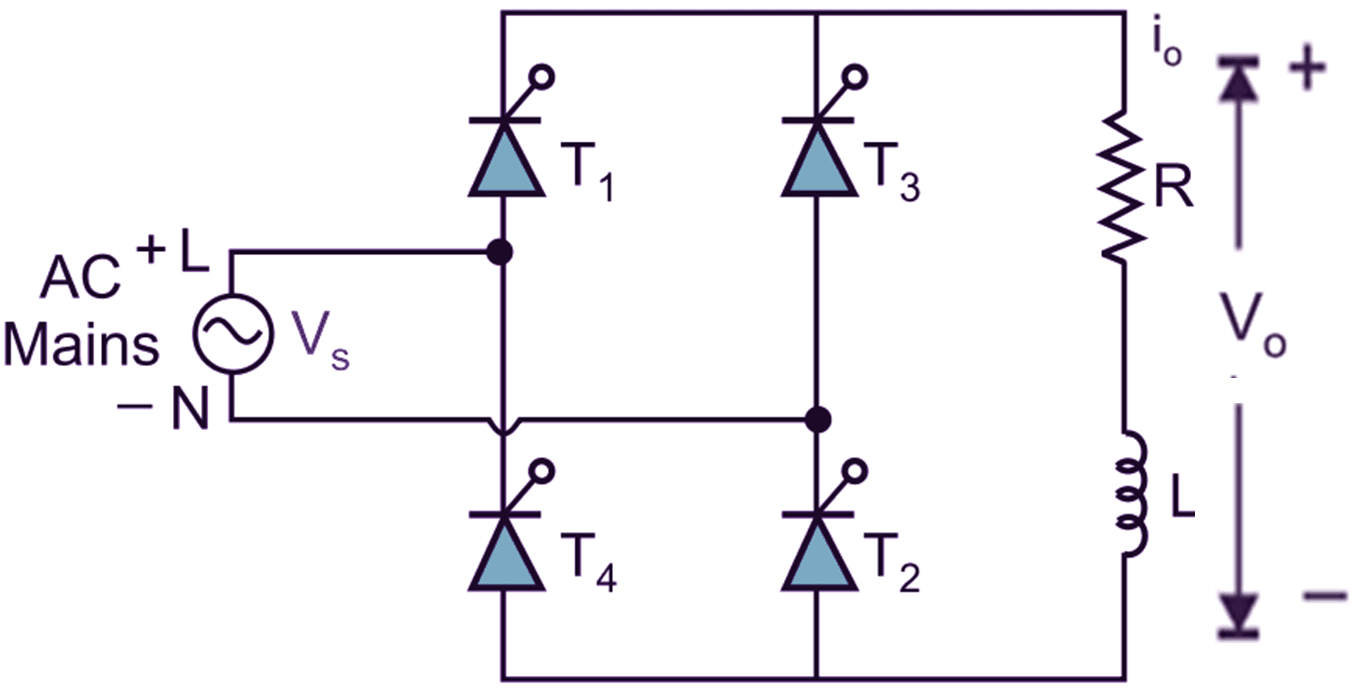
\includegraphics[width=0.7\textwidth]{Figures/single_phase_full_bridge_thyristor.png}
    \caption{Single-phase full bridge thyristor rectifier.}
    \label{fig:single_phase_thyristor_fb}
\end{figure}

\begin{figure}[H]
    \centering
    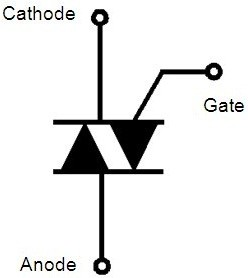
\includegraphics[width=0.2\textwidth]{Figures/triac_symbol.png}
    \caption{Back-to-back thyristors (triac).}
    \label{fig:triac}
\end{figure}

One can also use a diode rectifier (3-phase or single phase) before the DC-DC converter. In second case, only the DC-DC converter is controlled for the output voltage level. Since the maximum value of the desired output DC voltage is 180 V, a buck converter will be suitable for this case. However this topology works only in one quadrant due to the unavailability of negative duty cycles and one way allowance of the diode. To achieve the 4-quadrant operation, one alternative is the H-bridge coming after the diode rectifier. By adjusting the duty cycles of appropriate switches for desired quadrant of operation, one can drive the DC motor in all regions. Our motor drive will be designed to support 4-quadrant operation. Therefore, the topology which includes full-bridge diode rectifiers and H-bridge controller is selected to be implemented. Overall configuration of the design that will drive the DC motor is given in the Figure \ref{fig:overall_diagram}. In generation modes, armature current flowing to the driver will be dissapated through a chopper resistance which is also controlled by a switch to utilize its operation. \\


\subsection{Control Methodology}
We will use PWM (Pulse Width Modulation) signals to control the MOSFETs, which will control the average voltage seen in the output terminals. We will use a micro-controller to generate and regulate the PWM signals according to the user input and system state. To drive the MOSFETs with the micro-controller signals, we need to use gate driver circuits. We will use an Arduino controller (ATMegaxxx) as microcontroller, and commercial half-bridge gate drivers will be ordered and used directly to reduce the circuit design workload and have better performance. \\

To be able to soft-start the DC-motor, avoid the armature current ripple, and avoid high transient currents during reference input changes, we will need a closed loop control methodology between DC-motor terminal voltage and the duty cycles of the switches (MOSFETs). If we do not control the terminal voltage and apply PWMs with constant duty cycles, motor will experience huge amount of torques (inducing high currents on the armature) that will damage the DC-motor and decrease its lifetime. Figure \ref{fig:overall_diagram} shows the overall control topology of the DC-motor driver design. Overall, the design does not control the rectifier side of the motor drive, full-bridge diode rectifiers are used to rectify the AC input. Then the ripple at the DC-output will be suppressed by an appropriate shunt capacitor. To be able drive the DC-motor on the generating modes, team decided not to supply the energy to the grid side, since the design does not have an inverter that will generate AC to be supplied to the grid. Instead, there will be open terminals for chopper resistance that will dissipate the supplied power when the DC-machine operates in generating modes. And then, depending on the operation mode, the controller will send the required PWM duty cycles to the gate drivers of the switches. Detailed information about the closed loop controls of switches are given below.

\begin{figure}[H]
    \centering
    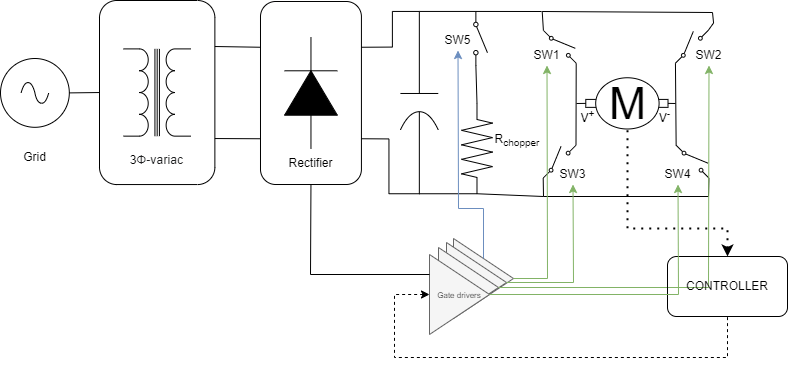
\includegraphics[width=0.8\textwidth]{Figures/topology_deneme.png}
    \caption{DC-motor drive system diagram.}
    \label{fig:overall_diagram}
\end{figure}

In our design, we plan to use closed-loop current control to control our driver by implementing a PID (Proportional Integral Derivative) controller. Since the armature current increases with increasing duty, it can be controlled by changing the duty cycles of the switches. The duty cycles will be adjusted using an error signal. By taking the discrete time derivative and integral of this error signal, we may obtain a discrete time PID controller. The equation for controlling the current by adjusting the duty cycle is given in Equation \ref{eqn:PID}.

\begin{equation}
    \begin{split}
        \Delta D = K_pE_{I_a} + K_i\sum_{n=1}^{t} E_{I_a}\Delta t + K_d\frac{\Delta E_{I_a}}{\Delta t}
    \end{split}
    \label{eqn:PID}
\end{equation}
\\
\subsection{Mechanical, Thermal, and Isolation Considerations}

In order to protect the DC-motor driver design from external incidents and achieve safer operation for users, the design will be enclosed in a 3D printed box. The size and shape of the box will be appropriate for industrial design applications. According the component sizes and PCB dimensions, smallest box volume will be selected and the DC-motor drive will be fixed in the volume. \\

Placement and connections of the components of the DC-motor drive will be solved on the PCB. This will prevent possible human-made errors and resulting parasitic effects on the circuit. It will also ease the industrial production of the design. \\

After the component selection and their trials during the implementation process, the conduction and switching losses will be calculated, compared with their simulation counterparts, then a proper-sized heatsink will be placed where the most of the heat losses occur on the circuit. \\

To prevent the motor driver circuit from possible loops that will endanger the operation of components, some isolation is required between the power flow lines and signal lines of the circuit and gate drivers. Therefore, the use of optocouplers are to be implemented on the design.

\subsection{Other Considerations}

To make the design available for easy use and proper testing, connection and measurement ports will be added to the design. According to the rated values (current and voltage) of the power lines, required isolation and line thicknesses will be implemented on both the connection ports and the PCB. For input power connection, proper sized banana plugs as seen in Figure \ref{fig:banana} can be selected. According to the connection style of DC-motor to be driven, again proper style of power cables for the output ports, will be selected.

\begin{figure}
    \centering
    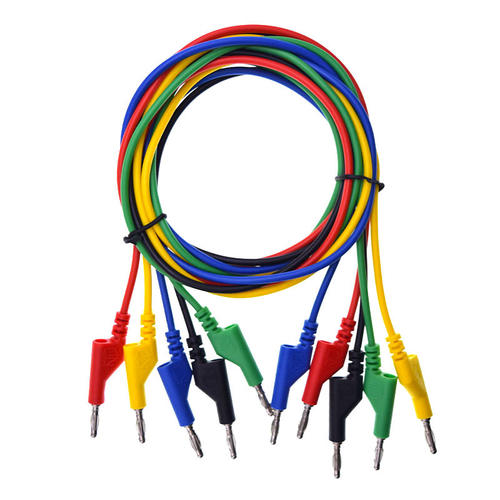
\includegraphics[width=0.4\textwidth]{Figures/banana plugs.jpg}
    \caption{Banana plug power cables for input side.}
    \label{fig:banana}
\end{figure}

For the measurement ports, the information on test procedures will be requested. Already selected ports for measurements are input and output voltages, ground connection of the motor drive. Since a series connection is requested for the electrical power calculations, it is assumed that power measurements will be taken before the input and output connections. If it is requested, the measurement ports for PWM signals of the gate drivers can be brought into the open. \\

To protect the components from over-voltages and over-currents during the operation, below measures can be applied to the design:

\begin{itemize}
    \item Fuses or current sensors at both the input and output sides of the driver circuit is thought to be implemented for over-current protection. If current sensors are to be implemented on the design, some alarm signal is to be presented to the user through some led or control method can be implemented to cut the power of the circuit.
    \item Since we are asked to supply around 2 kW power through the motor driver (excluding losses), we are dealing with high levels of current and power that can be harmful to a human body. Therefore, proper insulation will be placed on the power lines, ports, and around the equipment.
    \item To cancel the parasitic effects of the non-idealities of the components, proper countermeasures will be considered.
\end{itemize}